\chapter{Návrh}
\label{sec:de}

\section{Návrhový vzor MVC}

Struktura nadřazeného systému je vhodná k~použití návrhového vzoru MVC, tedy \textit{model-view-controller}. \textit{Model} zde představují garáže (podřízené systémy), k~nim vázané události a logika jejich vyhodnocování. 

\textit{View} je zobrazení těchto dat, tedy především generované HTML stránky webového rozhraní. Jako další \textit{view} je možné považovat získávání dat (například ve formátu JSON) pomocí API nadřazeného systému, třeba při zasílání registračních klíčů podřízeným systémům.

\textit{Controller} je pak část aplikace, která se stará o~zpracování HTTP požadavků. Ty mohou přicházet jednak z~uživateloval prohlížeče, jednak od podřízených systémů. Na základě těchto požadavků pak \textit{controller} posílá příslušné příkazy \textit{modelu}. Struktura aplikace při použití vzoru MVC je naznačena na obrázku \ref{fig:mvc}.

\begin{figure}[h!]
    \centering
    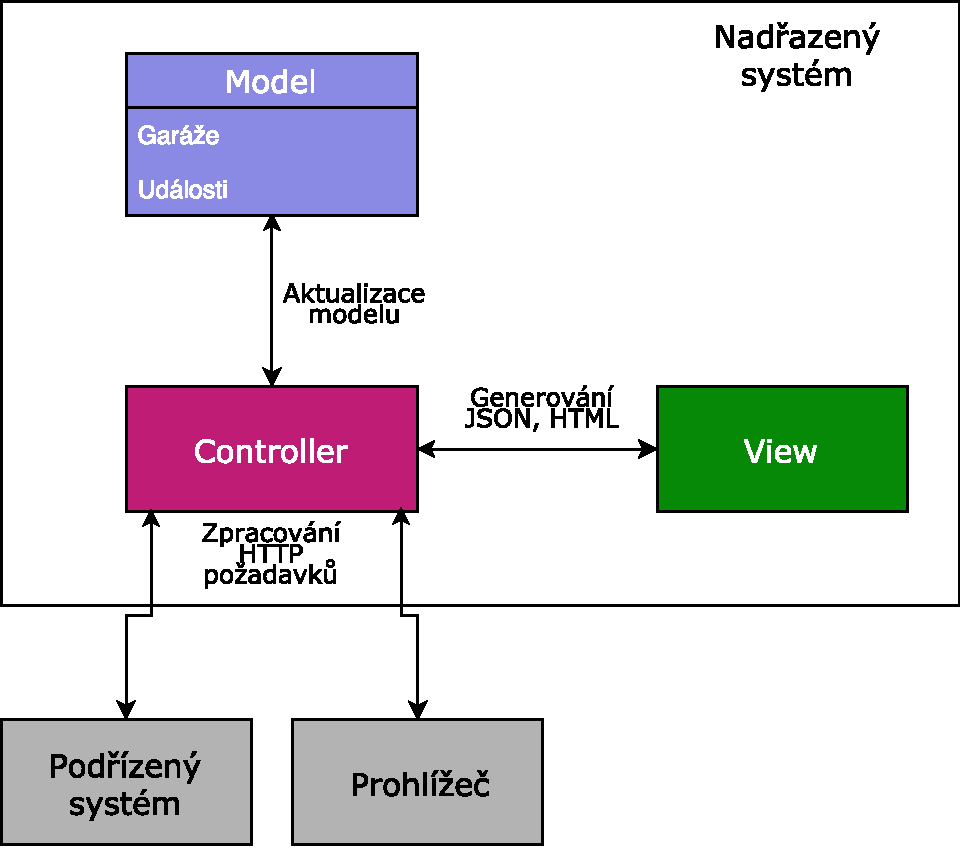
\includegraphics[width=0.7\textwidth]{images/mvc.pdf}
    \caption{Struktura MVC aplikace}
    \label{fig:mvc}
\end{figure}

Hlavní motivací pro použití tohoto vzoru je snadná rozšiřitelnost. Pokud by například bylo potřeba aplikaci doplnit o~komunikaci s~podřízenými systémy pomocí MQTT, stačí pouze vytvořit vhodný \textit{controller}. Ten pak může využívat \textit{model} aplikace stejným způsobem jako HTTP \textit{controller}.

\section{Flask Blueprints}

ta sekce s~blueprintama bude asi nejlepsi tady hned z~kraje

\url{http://flask.pocoo.org/docs/0.12/blueprints/}

rekneme ze budeme mit tri blueprinty (moduly):

\begin{itemize}
    \item main modul -- tady bude definovanej ten hlavni model, tj garaze, eventy a pripadne naka fasada na tim. Controller a view pak bude zprostredkovavat uzivatelsky rozhrani (krome loginu) webovy stranky. V~timhle rozhrani pude proklikavat ty garaze a eventy, zapinat registraci mod a vytvaret/mazat garaze. To vytvareni garazi je hlavne kvuli nakejm dev options, primarne se budou garaze vytvaret skrz to api (tj tim cudlikem na podrizenym systemu). Vytvorit garaz v~uzivatelskym rozhrani nebude vyzadovat zapnutej registracni mod, tj to bude uplne jinej pozadavek na uplnej jinej controller -- ten v~main modulu a ne v~api modulu
    \item api modul -- modul co bude zprostredkovavat api pro podrizeny systemy. tj tady se nebude generovat zadny html nebo veci pro uzivatelsky rozhrani, ale ciste jen zpracovavat pozadavky vod podrizenejch systemu. Modul bude vyuzivat tu fasadu z~main modulu pro pristup k~databazi (stejne jako main modul). Controller v~timhle modulu bude teda resit pozadavky na vytvareni novejch garazi pomoci API. To jestli je zapnutej registracni mod bude resit ten model, v~tim bude vodlisna funkce pro vytvoreni garaze pres reg. mod a pres rozhrani a prislusny controllery budou volat prislusnou funkci. Krome toho tenhle controller bude resit pozadavky na vytvoreni eventu.
    \item auth modul -- tenhle modul bude resit ciste prihlaseni uzivatele do webovyho rozhrani
\end{itemize}

Z~toho vypliva ze jadrem ty aplikace bude ten datovej model (garaze, eventy atd...) a fasada nad nim. Ta fasada by teda mela umet nasledujici veci (za pomlckou kterej modul to bude pouzivat):

\begin{itemize}
    \item vytvorit garaz (pozadavek z~web. rozhrani) -- main
    \item vytvorit garaz (pozadavek z~api -- tj kontrola reg. modu) -- api
    \item vypnout/zapnout reg. mod -- main
    \item smazat garaz -- main
    \item vratit vsechny garaze -- main
    \item vratit konkretni garaz -- main, (api?)
    \item vratit vsechny eventy -- main
    \item vratit eventy ke garazi -- main
    \item vytvorit event vazanej ke garazi -- api
    \item kontrola klicu pozadavku vod api -- api
    \item vnitrni udrzovani stavu garazi a vyhodnocovani udalosti -- main, api
\end{itemize}

\section{Model}

pouziti sqlalchemy -- to resit az v~implementaci

\subsection{Garáž}

\subsubsection{Stav garáže}

\subsection{Událost}

\subsubsection{Vyhodnocení události}

\subsection{Fasáda}

\section{Controller}

Flask API

\section{View}

\section{Autentizace}

\subsection{Autentizace uživatele}

\subsection{Autentizace podřízeného systému}

\subsubsection{Registrační mód}

\subsection{API}
